\section{FineGrainedTree}
\label{finegrainedtree}

This kind of structure is basically the same discussed in \ref{coarsegrainedtree}; the main difference between theese two structures, is the use of the locks.

Putting a lock for each node of the tree means to complicate the management of the whole structure in favor of the possibility to work concurrently on the tree for more than one thread and reduces lock contention.
\newline 

Like in the FineGrainedList structure, described in \ref{finegrainedlist}, we need to add to each node a Boolean marked field indicating whether that node is in the set; by doing this, we avoid problems like the attempt of a thread to add a node as a child of a node that another thread wants to remove.
\newline

Taking in account what discussed above, the new element of the tree can be represented as following:\newline

\begin{lstlisting}
	class Node<T>{
		boolean marked;
		Lock lock;
		T value;
		Node<T> left;
		Node<T> right;
	}
\end{lstlisting}

For the same reasons discussed in \ref{finegrainedlist} we need a \emph{validation} method that has to check the actual status of the lock elements.
\newline

To add a new element in the tree, a thread must acquire the lock on the node that will become the parent of the new node.
If the new element is already present in the tree and if the node with the same value already has a left child, the thread must acquire the lock on both nodes.
\newline

The \emph{remove} method has to acquire the right number of locks (depending on the position of the node), from the parent of the target node until is needed;
than the method has to mark the target node, logically removing it, and than redirects all the pointers needed as in a standard BST delection, physically removing the node.

It is important also in this case that all the locks must be acquired in the same order from all the thread, otherwise the deadlock is inevitable.

By doing this, the method has to acquire a number of locks between 2 (the best case in which the target node is a leaf) and $\log d$ where d is the depth of the first left leaf in the right subtree (or viceversa).

\begin{figure}
	\centering
	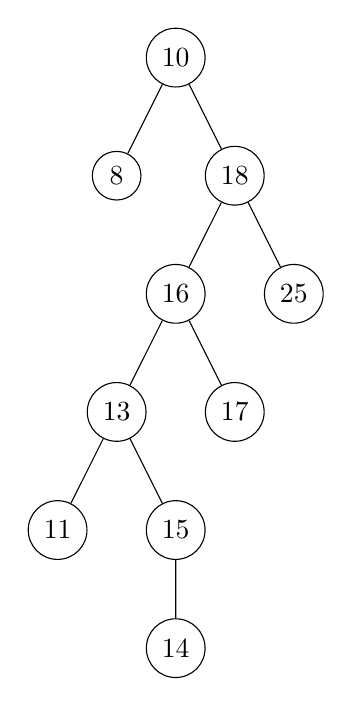
\begin{tikzpicture}
	    \tikzstyle{every node}=[circle,draw]
	    \node {10}
	        child { node {8} }
	        child {
	            node {18}
	            child { 
	            		node {16}
	            		child{
	            			node{13}
	            			child{ node{11} }
	            			child{ 
	            				node{15}
	            				child{ node{14} }
	            			}
	            		}
	            		child{ node {17} }
	            	}
	            child { node {25} }
	        }
	    ;
	\end{tikzpicture}
	\caption{Example of the worst case}
	\label{fig:badTree}
\end{figure}

Obviously this kind of use of the locks, leads to a degradation of the performance (especially if the structure is not well populated with respect to the number of threads).
\newline

There are some kinds of fix like marking the node that has been deleted as rooted, without phisically removing it, but then we will need also a method for checking if a rooted node can be phisically removed (sooner or later should be removed) and also a method to rebalance the tree in case it becomes too unbalanced.

As discussed in \ref{finegrainedlist}, the method \emph{toString} has to acquire the lock only on the current node (if it not marked) but also in this case, the structure that will be printed could be not the real status of it but only a partial one, since it can be modified meanwhile.
The order in which the node are printed is the same described in \ref{coarsegrainedtree}.
\newline

However the performance with respect to CoarseGrainedTree are improved in terms of concurrency, but the methods are still not wait-free.